%!TEX root = algebra.tex

\chapter{Grupos} % (fold)
\label{cha:Grupos}


Texto introdut\'orio\todo[size=\small, color=green!40]{Motiva\c{c}\~ao sobre grupos.}%


\section{Defini{\c c}{\~a}o e Propriedades}% (fold)
\label{sec:definicao_e_propriedades}
\begin{definicao}
	Um \textbf{grupo} $G$ {\'e} um conjunto n{\~a}o vazio munido com uma opera{\c c}{\~a}o bin{\'a}ria $*$ tal que\index{Grupos}
	\begin{enumerate}[label=({\roman*})]
		\item Para todo $x$, $y$, $z\in G$: $(x*y)*z=x*(y*z)$, isto \'e, a opera\c{c}\~ao $*$ \'e associativa.\index{Grupos!Associatividade}
		\item Existe $e\in G$ tal que $x*e=e*x=x$ para todo $x\in G$. Tal elemento $E$ {\'e} chamado de \textbf{elemento neutro} ou \textbf{unidade}.\index{Grupos!Elemento neutro}
		\item Para cada $x\in G$, existe $y\in G$ tal que $x*y=y*x=e$. O elemento $y$ {\'e} chamado de \textbf{inverso} de $x$ e \'e denotado por $y = x^{-1}$.\index{Grupos!Inverso}
	\end{enumerate}
\end{definicao}

Denotamos um grupo $G$, cuja opera{\c c}{\~a}o bin{\'a}ria {\'e} $*$, por $(G,*)$. Quando $*$ {\'e} a soma, dizemos que $(G,*)$ {\'e} um grupo aditivo. Se $*$ {\'e} a multiplica{\c c}{\~a}o, dizemos que $(G,*)$ {\'e} um grupo multiplicativo. Caso n\~ao haja possibilidade de confus\~ao em rela\c{c}\~ao \`a opera\c{c}\~ao do grupo, diremos simplesmente que $G$ \'e um grupo.

\begin{observacao}
	Para simplificar a nota\c{c}\~ao vamos escrever $x * y = xy$ para $x$ e $y$ elementos de um grupo $(G, *)$.
\end{observacao}
\begin{definicao}Um grupo $(G,*)$ {\'e} chamado de \textbf{grupo comutativo} ou \textbf{abeliano} quando a opera\c{c}\~ao $*$ {\'e} comutativa, ou seja, $x*y=y*x$ para todo $x$, $y\in G$.\index{Grupos!Abelianos}
\end{definicao}

\begin{exemplos}
	\begin{enumerate}[label=({\arabic*})]
		\item Grupos aditivos: $\Z$, $\Q$, $\R$, $\comp$.
		\item $(M_n(K), +)$ \'e um grupo abeliano;
		\item $(GL_n(K), \cdot)$, onde $K$ \'e um corpo e $GL_n(K)$ denota as matrizes invert{\'\i}veis com entradas em $K$. $GL_n(K)$ n\~ao \'e um grupo abeliano.
		\item Seja $X$ um conjunto n\~ao vazio. Denote por $S_X = \{\sigma : X \to X \mid \sigma \mbox{ \'e uma bije\c{c}\~ao}\}$. O conjunto $S_X$ com a composi\c{c}\~ao de fun\c{c}\~oes \'e um grupo. No caso em que $X = \{1, 2, \dots, n\}$, obtemos $S_n = \{(1), (12), (13), (23), (123), \dots, (123\cdots n)\}$ o grupo das permuta\c{c}\~oes em $n$ elementos. Em geral, $S_X$ n\~ao \'e abeliano.
		\item Para qualquer inteiro $n$ seja
		\[
			\mu_n = \{\zeta^k : 0 \le k \le n\}
		\]
		onde $\zeta = e^{2\pi i/n} = \cos(2\pi/n) + i\sin(2\pi/n)$. Ent\~ao $\mu_n$ \'e um grupo abeliano multiplicativo.
		\item Seja $X$ um conjunto. Se $U$ e $V$ s\~ao subconjuntos de X defina
		\[
			U - V = \{x \in U \mid x \notin V\}.
		\]
		O \textbf{grupo Boleano} $\mathcal{B}(X)$ \'e a fam{\'\i}lia de todos os subconjuntos de $X$ munido da \textbf{adi\c{c}\~ao sim\'etrica} $A + B$ onde
		\[
			A + B = (A - B) \cup (B - A).
		\]
		\begin{figure}[h]
			\centering
			\caption{A soma $A + B$ \'e representada pela \'area em azul:}
			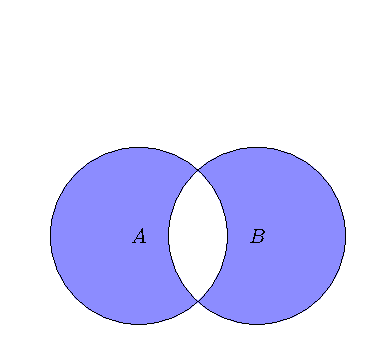
\includegraphics{grupo-boleano.pdf}
		\end{figure}

		\begin{figure}[h]
			\centering
			\caption{A associatividade \'e representada pela \'area em azul:}
			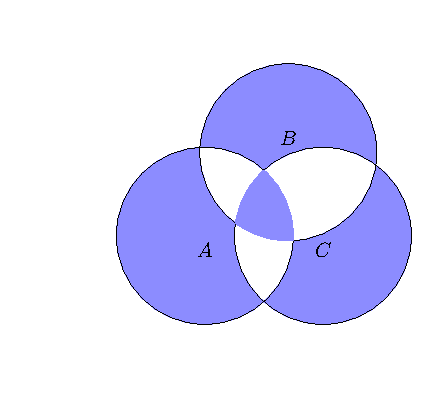
\includegraphics{grupo-boleano-associatividade.pdf}
		\end{figure}
		Assim $\mathcal{B}(X)$ \'e um grupo comutativo, o elemento neutro e $\emptyset$ e $A^{-1} = A$ pois $A + A = \emptyset$.
	\end{enumerate}
\end{exemplos}

\begin{lema}
Seja $(G,*)$ um grupo.
\begin{enumerate}[label=({\roman*})]
\item Vale a lei do cancelamento: se $x * a = x * b$ ou $a * x = b * x$, ent\~ao $a = b$.
\item O elemento neutro {\'e} {\'u}nico.
\item Existe um {\'u}nico inverso para cada $x\in G$.
\item Para todos $x$, $y\in G$ temos $(x*y)^{-1}=y^{-1}*x^{-1}$. Por indu{\c c}{\~a}o, $x_{1}$, $x_{2}$, \dots $x_{n-1}$, $x_{n}\in G$
	\[
		(x_1*x_2*...*x_{n-1}*x_n)^{-1} = x^{-1}_n*x^{-1}_{n-1}*...*x^{-1}_2*x^{-1}_1.
	\]
\item Para todo $x\in G, (x^{-1})^{-1}=x$.
\end{enumerate}
\end{lema}

\begin{definicao}
	Se $G$ \'e um grupo e se $a \in G$, defina as \textbf{pot\^encias} $a^n$, para $n \ge 1$, como sendo\index{Grupos!Pot\^encias de um elemento}
	\[
		a^1 = a\quad \mbox{e}\quad a^{n + 1} = a^na.
	\]
	Definimos $a^0 = 1$ e se $n$ \'e um inteiro positivo, definimos
	\[
		a^{-n} = (a^{-1})^n.
	\]
\end{definicao}

\begin{lema}
	Se $G$ \'e um grupo e $a$, $b \in G$, ent\~ao $(ab)^{-1} = b^{-1}a^{-1}$.
\end{lema}

\begin{lema}
	Sejam $G$ um grupo, $a$, $b \in G$ e $m$, $n \ge 1$. Ent\~ao
	\begin{align*}
		a^{m + n} = a^ma^n\\
		(a^m)^n = a^{mn}.
	\end{align*}
\end{lema}

\begin{proposicao}
	Sejam $G$ um grupo, $a$, $b \in G$ e $m$, $n \in \Z$.
	\begin{enumerate}[label=({\roman*})]
		\item Se $a$ e $b$ comutam, ent\~ao $(ab)^n = a^nb^n$.
		\item $(a^m)^n = a^{mn}$
		\item $a^ma^n = a^{m + n}$ 
	\end{enumerate}
\end{proposicao}

\begin{definicao}
	Seja $G$ um grupo e $a \in G$. Se $a^k = 1$ para algum $k \ge 1$, ent\~ao o menor expoente $k \ge 1$ \'e chamado de \textbf{ordem} de $a$. Se n\~ao existe tal pot\^encia, dizemos que $a$ tem \textbf{ordem infinita}.\index{Ordem!de elemento}
\end{definicao}

\begin{teorema}\label{ordem_elemento}
	Se $a \in G$ \'e um elemento de ordem $n$, ent\~ao $a^m = 1$ se, e somente se, $n | m$.
\end{teorema}
\begin{prova}
	Suponha que $a^m = 1$. Assim pelo Algor{\'\i}tmo da Divis\~ao de Euclides, existem inteiros $q$ e $r$ tais que
	\[
		a^m = a^{nq + r}
	\]
	onde $0 \le r \le n$. Assim
	\[
		a^r = a^ma^{-nq} = 1.
	\]
	Se $r > 0$, obtemos uma contradi\c{c}\~ao com a ordem de $a$. Logo $r = 0$ e portanto $n | m$. Agora, se $n | m$, ent\~ao
	\[
		a^m = a^{nq} = 1
	\]
	como quer{\'\i}amos.
\end{prova}

\begin{proposicao}
	Se $G$ \'e um grupo finito, ent\~ao todo $x \in G$ tem ordem finita.
\end{proposicao}
\begin{prova}
	Seja $x \in G$. Considere o conjunto $\{1, x, x^2, \dots, x^n,\dots\}$. Como $G$ \'e finito, existem inteiros $m > n$ tais que $x^m = x^n$, isto \'e, $x^{m - n} = 1$. Portanto $x$ tem ordem finita.
\end{prova}

% section definicao_e_propriedades (end)

\section{Subgrupos} % (fold)
\label{sec:subgrupos}
\begin{definicao}
	Seja $(G, \cdot)$. Um conjunto n\~ao vazio $H$ de $G$ \'e um \textbf{subgrupo}, que denotaremos por $H \le G$, quando com a opera\c{c}\~ao de $G$, o conjunto $H$ \'e um grupo, isto \'e, quando as condi\c{c}\~oes seguintes s\~ao satisfeitas:\index{Subgrupos}
	\begin{enumerate}[label=({\roman*})]
		\item $h_1h_2 \in H$ para todos $h_1$, $h_2 \in H$;
		\item $1 \in H$;
		\item Se $x \in H$, ent\~ao $x^{-1} \in H$.
	\end{enumerate}
\end{definicao}

\begin{proposicao}
	Um subconjunto $H$ de um grupo $G$ \'e um subgrupo se, e somente se, $H$ \'e n\~ao vazio e para quaisquer $x$, $y \in H$ temos $xy^{-1} \in H$.
\end{proposicao}
\begin{prova}
	A ida \'e imediata. Agora, suponha que $H$ n\~ao \'e vazio e que $xy^{-1} \in H$ para todos $x$, $y \in H$. Assim tomando $x \in H$ temos $1 = xx^{-1} \in H$. Se $y \in H$, ent\~ao $y^{-1} = 1y^{-1} \in H$ e finalmente se $x$ e $y \in H$, ent\~ao $xy = x(y^{-1})^{-1} \in H$. Portanto $H$ \'e um subgrupo de $G$.
\end{prova}

\begin{exemplos}
	\begin{enumerate}[label=({\arabic*})]
		\item Se $G$ \'e um grupo, ent\~ao $\{1\}$ e $G$ s\~ao subgrupos de $G$ chamados de \textbf{trivias}.\index{Grupos!Triviais}
		\item $(2\Z,+)$ \'e um subgrupo de $(\Z,+)$. De maneira geral, se $n$ \'e um inteiro qualquer, ent\~ao $(n\Z,+)$ \'e um subgrupo de $(\Z,+)$.
		\item O conjunto $V = \{(1), (12)(34), (13)(24), (14)(23)\}$ \'e um subgrupo de $S_4$.
		\item Seja $G$ um grupo qualquer. COnsidere o subconjunto
		\[
			Z(G) = \{x \in G \mid xg = gx\ \mbox{para todo } g \in G\}.
		\]
		Mostre que $Z(G) \le G$. Este subgrupo $Z(G)$ \'e chamado de \textbf{centro} de $G$. O grupo $G$ \'e abeliano se, e s\'o se, $Z(G) = G$.\index{Grupos!Centro}
	\end{enumerate}
\end{exemplos}

\begin{proposicao}\label{subgrupo_em_grupos_finitos}
	Um conjunto n\~ao vazio de um grupo finito $G$ \'e um subgrupo de $G$ se, e somente se, $H$ \'e fechado, isto \'e, se dados $a$ e $b \in H$, ent\~ao $ab \in H$. Em particular, um subconjunto n\~ao vazio de $S_n$ \'e um subgrupo se, e somente se, \'e fechado.
\end{proposicao}
\begin{prova}
	A ida \'e imediata. Para a volta, como $G$ \'e finito todos os seus elementos t\^em ordem finita. Dado $x \in H$, ent\~ao existe um inteiro $n$ tal que $x^n = 1$. Assim $1 \in H$, pois $H$ \'e fechado. Al\'em disso, $x^{-1} = x^{n - 1} \in H$. Finalmente, se $x$ e $y \in H$, ent\~ao $xy^{-1} = xy^{m - 1} \in H$, onde $m$ \'e um inteiro tal que $y^m = 1$. Portanto $H$ \'e um subgrupo de $G$.
\end{prova}

\begin{observacoes}
	\begin{enumerate}[label=({\arabic*})]
		\item A Proposi\c{c}\~ao \ref{subgrupo_em_grupos_finitos} pode falhar se $G$ for um grupo infinito. Por exemplo, seja $G = \Z$ o grupo aditivo dos inteiros. O conjunto $H = \N$ \'e fechado, mas n\~ao \'e um subgrupo de $\Z$.
		\item Para Galois, 1830, um grupo era simplesmente um conjunto fechado $H$ de $S_n$. Foi A. Cayley, em 1854 o primeiro a definir um grupo abstrato mencionando explicitamente a associatividade, o inverso e elemento neutro.
	\end{enumerate}
\end{observacoes}

Vamos fixar algumas nota\c{c}\~oes: se $H$ e $K$ s\~ao subconjuntos de um grupo $G$ (em particular, se $H$ e $K$ s\~ao subgrupos de $G$) definimos
\begin{align*}
	HK = \{hk \mid h \in H\, k \in K\}\\
	H^{-1} = \{h^{-1} \mid h \in H\}.
\end{align*}

Em geral $HK$ n\~ao \'e um subgrupo de $G$, mesmo quando $H$ e $K$ o s\~ao. (Apresente alguns exemplos!)

Dado um subconjunto n\~ao vazio $S$ de $G$, denotamos
\[
	\ger{S} = \{a_1\dots a_n \mid n \in \N, a_i \in S \mbox{ ou } a_i \in S^{-1}\}.
\]
Quando o conjunto $S$ for finito, digamos $S = \{a_1, \dots, a_n\}$ escreveremos
\[
	\ger{\{a_1,\dots, a_n\}} = \ger{a_1,\dots,a_n}.
\]
Quando $g \in G$ escrevemos
\[
	\ger{g} = \{\dots, g^{-2}, g^{-1}, 1, g, g^2,\dots\} = \{g^t \mid t \in \Z\}.
\]

\begin{proposicao}
	Sejam $G$ um grupo e $S$ um subconjunto n\~ao vazio de $G$. Ent\~ao o conjunto $\ger{S}$ \'e um subgrupo de $G$.
\end{proposicao}
\begin{prova}
	Como $S \ne \emptyset$, ent\~ao $1 \in \ger{S}$. Dados $x$, $y \in S$ temos
	\begin{align*}
		x = a_1a_2\dots a_m\\
		y = b_1b_2\dots b_n\\
	\end{align*}
	com $a_i$, $b_j \in S$ ou $a_i$, $b_j \in S^{-1}$ para todo $i$ e todo $j$. Logo $y^{-1} = b_n^{-1}\dots b_2^{-1}b_1^{-1}$ para todo $j$, da{\'\i}
	\[
		xy^{-1} = a_1\dots a_mb_{n}^{-1}\dots b_2^{-1}b_1^{-1} \in \ger{S}.
	\]
	Portanto $\ger{S}$ \'e um subgrupo de $G$.
\end{prova}

\begin{definicao}
	Sejam $G$ um grupo e $S$ um subconjunto n\~ao vazio de $G$. Ent\~ao $\ger{S}$ \'e chamado de \textbf{subgrupo gerado} por $S$.\index{Subgrupos!gerados por um conjunto}
\end{definicao}

\begin{definicao}
	Um grupo \'e \textbf{c{\'\i}clico} quando ele pode ser gerado por um elemnto, isto \'e, quando $G = \ger{g}$ para algum $g \in G$.\index{Grupos!C{\'\i}clicos}
\end{definicao}

\begin{definicao}
	A \textbf{ordem} de um grupo $G$ \'e o n\'umero de elementos em $G$.\index{Grupos!Ordem}
\end{definicao}

\begin{proposicao}
	Resultado sobre ordem de elemento.
\end{proposicao}

\begin{teorema}
	Se $G = \ger{a}$ \'e um grupo c{\'\i}clico de ordem $n$, ent\~ao $a^k$ \'e um gerador de $G$ se, e somente se, $mdc(k,n) = 1$.
\end{teorema}
\begin{prova}
	Se $a^k$ \'e um gerador de $G$, ent\~ao $a = a^{kt}$ para algum $t \in \Z$. Da{\'\i} $a^{kt - 1} = 1$ e ent\~ao pelo Teorema \ref{ordem_elemento}, $n | (kt -1)$, isto \'e, $nu = kt - 1$ para algum $u \in \Z$. Logo, $mdc(k,n) = 1$.

	Agora, se $mdc(k,n) = 1$, ent\~ao existem $p$, $q \in \Z$ tais que $kp + nq = 1$. Da{\'\i}
	\[
		a = a^{kp + nq} = a^{nq}(a^k)^p = (a^k)^p
	\]
	e ent\~ao $G = \ger{a}$.
\end{prova}

\begin{proposicao}\label{ordem_de_elemento}
	Seja $G$ um grupo finito e seja $a \in G$. Ent\~ao a ordem de $a$ \'e igual ao n\'umero de elementos em $\ger{a}$, ou seja,
	\[
		|a| = |\ger{a}|.
	\]
\end{proposicao}
\begin{prova}
	Como $G$ \'e finito, existe um inteiro $k \ge 1$ tal que o conjunto $\{1, a, a^2, \dots, a^{k - 1}\}$ cont\'em todos os elementos distintos de $G$, enquanto na lista $1$, $a$, $a^2$, \dots, $a^k$ possui elementos repetidos. Da{\'\i} $a^k \in \{1, a, a^2, \dots, a^{k - 1}\}$. Assim $a^k = a^i$ para algum $i$ com $0 \le i \le k - 1$. Se $i \ge 1$, ent\~ao $a^{k - i} = 1$, o que contradiz o fato de que n\~ao h\'a repeti\c{c}\~oes entre os elementos $1$, $a$, $a^2$, \dots, $a^{k - 1}$. Logo $a^k = a^0 = 1$ e assim $k$ \'e a ordem de $a$.

	Se $H = \{1, a, a^2, \dots, a^{k - 1}\}$, ent\~ao $|H| = k$. Assim \'e suficiente provar que $H = \ger{a}$. Claramente $H \sub \ger{a}$. Agora seja $a^i \in \ger{a}$. Pelo Algor{\'\i}tmo da Divis\~ao de Euclides, existem $q$ e $r \in \Z$ tais que $i = qk + r$, onde $0 \le r \le k$. Assim $a^i = a^{qk}a^r = a^r \in H$, isto \'e, $\ger{a} \sub H$. Portanto, $H = \ger{a}$.
\end{prova}

\begin{definicao}
	O subgrupo $\ger{\{xyx^{-1}y^{-1} \mid x, y \in G\}}$ \'e o \textbf{subgrupo dos comutadores} do grupo $G$. Ele ser\'a denotado por $G'$. Note que $G$ \'e abeliano se, e somente se, $G' = \{1\}$.\index{Subgrupos!dos comutadores}
\end{definicao}


% section subgrupos (end)

\section{Teorema de Lagrange} % (fold)
\label{sec:teorema_de_lagrange}

Sejam $G$ um grupo e $H$ um subgrupo de $G$. Sobre $G$ defina a rela\c{c}\~ao $\sim_{E}$ da seguinte maneira
\[
	y \sim_{E} x \mbox{ se, e somente se, exite } h \in H \mbox{ tal que } y = xh.
\]
\'E imediato verificar que $\sim_{E}$ \'e uma rela\c{c}\~ao de equival\^encia. Dado $x \in G$ a classe de equival\^encia de $x$ \'e o conjunto
\[
	xH = \{y \in G \mid y \sim_{E} x\} = \{xh \mid h \in H\}
\]
que chamaremos de \textbf{classe lateral \`a esquerda} de $H$ em $G$. Quando n\~ao houver chance de confus\~ao, diremos simplesmente classe lateral de $x$ \`a esquerda. Observe que $y \in xH$ se, e s\'o se, $yH = xH$.\index{Grupos!classe lateral \`a esquerda}

Analogamente, podemos definir a seguinte rela\c{c}\~ao de equival\^encia:
\[
	y \sim_{D} x \mbox{ se, e somente se, exite } h \in H \mbox{ tal que } y = hx. 
\]
Obtemos assim as \textbf{classes laterais \`a direita} de $H$ em $G$. A classe lateral de $x$ \`a direita \'e dada por\index{Grupos!classe lateral \`a direita}
\[
	Hx = \{y \in G \mid y \sim_{D} x\} = \{hx \mid h \in H\}.
\]

\begin{definicao}
	Dado um grupo $G$ e $H$ um subgrupo de $G$, o conjunto das classes laterais \`a esquerda de $H$ em $G$ \'e denotado por
	\[
		\left(\dfrac{G}{H}\right)_E = \{xH \mid x \in G\}.
	\]
	Analogamente, definimos
	\[
		\left(\dfrac{G}{H}\right)_D = \{Hy \mid y \in G\}.
	\]
\end{definicao}

\begin{definicao}
	A cardinalidade do conjunto das classes laterais \`a esquerda, $(G/H)_E$, \'e o \textbf{{\'\i}ndice} de $H$ em $G$ e ser\'a denotado por $[G:H]$.\index{Grupos!{\'\i}ndice}
\end{definicao}

\begin{observacao}
	O {\'\i}ndice de $H$ em $G$ tamb\'em \'e a cardinalidade do conjunto das classes laterais \`a direita de $H$ em $G$. De fato, \'e imediato verificar que a aplica\c{c}\~ao
	\begin{align*}
		\varphi : \left(\dfrac{G}{H}\right)_E \to \left(\dfrac{G}{H}\right)_D\\
		xH \mapsto Hx^{-1}
	\end{align*}
	est\'a bem definida e \'e uma bije\c{c}\~ao.
\end{observacao}

\begin{proposicao}
	Todas as classes laterais de $H$ em $G$ t\^em a mesma cardinalidade, igual \`a cardinalidade de $H$.
\end{proposicao}
\begin{prova}
	Basta verificar que a aplica\c{c}\~ao
	\begin{align*}
		\varphi : H \to \left(\dfrac{G}{H}\right)_E\\
		x \mapsto xH
	\end{align*}
	\'e uma bije\c{c}\~ao.
\end{prova}

\begin{teorema}[Teorema de Lagrange]\label{teorema_de_lagrange}
	Sejam $G$ um grupo finito e $H$ um subgrupo de $G$. Ent\~ao
	\[
		|G| = |H|[G:H],
	\]
	em particular, a ordem e o {\'\i}ndice de $H$ dividem a ordem de $G$.
\end{teorema}
\begin{prova}
	Seja $\{a_1H, a_2H, \dots, a_tH\}$ a fam{\'\i}lia de todas as classes laterais distintas de $H$ em $G$. Ent\~ao
	\[
		G = a_1H \cup a_2H \cup \cdots \cup a_tH
	\]
	e assim
	\[
		|G| = |a_1H| + |a_2H| + \cdots + |a_tH|.
	\]
	Mas, $|H| = |a_iH|$ para todo $i = 1$, \dots, $t$, onde $t = [G:H]$. Portanto
	\[
		|G| = |H|[G:H]
	\]
	como quer{\'\i}amos.
\end{prova}

\begin{corolario}\label{primeiro_corolario_lagrange}
	Sejam $G$ um grupo finito e $\alpha \in G$. Ent\~ao a ordem de $\alpha$ divide a ordem de $G$.
\end{corolario}
\begin{prova}
	Segue da Proposi\c{c}\~ao \ref{ordem_de_elemento} pois $|\alpha| = |\ger{\alpha}|$.
\end{prova}

\begin{corolario}
	Se $G$ \'e um grupo finito, ent\~ao $a^{|G|} = 1$ para todo $a \in G$.
\end{corolario}
\begin{prova}
	Se $a$ possui ordem, ent\~ao pelo Corol\'ario \ref{primeiro_corolario_lagrange}, devemos ter $|G| = dm$ para algum $m \ge 1$. Logo $a^{|G|} = a^{dm} = 1$.
\end{prova}

\begin{corolario}
	Se $p$ \'e um n\'umero primo, ent\~ao todo grupo $G$ de ordem $p$ \'e c{\'\i}clico.
\end{corolario}
\begin{prova}
	Se $a \in G$, $a \ne 1$, ent\~ao $a$ tem ordem $d > 1$, o que \'e imposs{\'\i}vel. Logo $G = \ger{a}$.
\end{prova}

\begin{proposicao}
	Seja $G$ um grupo abeliano.
	\begin{enumerate}[label=({\roman*})]
		\item Se $a$, $b \in G$ s\~ao dois elementos de ordem finita tais que $mdc\{|a|, |b|\} = 1$, ent\~ao $|ab| = |a||b|$.
		\item Se $r:= sup\{|g| \mid g \in G\}$ \'e finito, ent\~ao $|x|$ divide $r$ para cada $x \in G$.
	\end{enumerate}
\end{proposicao}
\begin{prova}
	\begin{enumerate}[label=({\roman*})]
		\item Sejam $|a| = m$, $|b| = n$ e $z = |ab|$. Como $a$ e $b$ comutam, temos $(ab)^{mn} = (a^m)^n(b^n)^m = 1$. Logo $z$ \'e um divisor de $mn$. Agora, $(ab)^z = 1$, da{\'\i} $a^z = b^{-z} \in \ger{a}\cap\ger{b}$. Mas $mdc(m,n) = 1$, logo $\ger{a}\cap\ger{b} = \{1\}$. Ent\~ao $a^z = b^z = 1$ e portanto $z$ \'e um m\'ultiplo de $m$ e de $n$. Como $m$ e $n$ s\~ao relativamente primos, $z$ \'e um m\'ultiplo de $mn$. Portanto, $z = mn$ como quer{\'\i}amos.
		\item Inicialmente vamos provas a seguinte afirma\c{c}\~ao:

		``Se $a$, $b \in G$ s\~ao dois elementos de ordem finita, ent\~ao existe $c \in G$ tal que $|c| = mmc\{|a|, |b|\}$.''

		Sejam $m = |a|$ e $n = |b|$. Se $mdc(m, n) = 1$, ent\~ao pelo item anterior podemos tomar $c = ab$. Se $mdc(m, n) \ne 1$, escreva
		\begin{align*}
			m = p_1^{\alpha_1}\cdots p_k^{\alpha_k}p_{k + 1}^{\alpha_{k + 1}}\cdots p_t^{\alpha_t}\\
			m = p_1^{\beta_1}\cdots p_k^{\beta_k}p_{k + 1}^{\beta_{k + 1}}\cdots p_t^{\beta_t}
		\end{align*}
		onde $0 \le \alpha_i < \beta_i$ para $i = 1$, \dots, $k$, $\alpha_j \ge \beta_j \ge 0$ para $j = k + 1$, \dots, $t$ e os primos $p_i$ s\~ao todos distintos.

		Considere os elementos
		\begin{align*}
			a_1 = a^{p_1^{\alpha_1}\cdots p_k^{\alpha_k}}\\
			b_1 = b^{p_{k + 1}^{\beta_{k + 1}}\cdots p_t^{\beta_t}}.
		\end{align*}
		Assim
		\begin{align*}
			|a_1| = p_{k + 1}^{\alpha_{k + 1}}\cdots p_t^{\alpha_t}\\
			|b_1| = p_1^{\beta_1}\cdots p_k^{\beta_k}.
		\end{align*}
		e ent\~ao $mdc\{|a_1|, |b_1|\} = 1$  e pelo item anterior basta tomar $c = a_1b_1$. Logo a afirma\c{c}\~ao est\'a provada.

		Para provar o item b), suponha que $r := sup\{|g| \mid g \in G\}$ \'e finito e tome $y \in G$ tal que $|y| = r$. Suponha que existe $x \in G$ tal que $|x|$ n\~ao divide $|y|$. Assim $s = mdc\{|x|, |y|\} > r$ e pela afirma\c{c}\~ao anterior existe $x \in \ger{x, y} \sub G$ tal que $|c| = s > r$, o que contradiz a defini\c{c}\~ao de $r$.
	\end{enumerate}
\end{prova}

\begin{proposicao}
	Seja $G$ um grupo e sejam $K < H < G$. Ent\~ao
	\[
		[G:K] = [G:H][H:K].
	\]
\end{proposicao}
% section teorema_de_lagrange (end)

\section{Subgrupos Normais e Grupos Quocientes} % (fold)
\label{sec:subgrupos_normais_e_grupos_quocientes}

Sejam $G$ um grupo e $H$ um subgrupo de $G$. Considere o conjunto das classes laterais \`a esquerda de $H$ em $G$:
\[
	\left(\dfrac{G}{H}\right) = \{xh \mid x \in G\}.
\]
Queremos definir uma opera\c{c}\~ao em $G/H$ de modo que este conjunto se torne um grupo. O meio natural de fazer isso \'e definindo
\begin{align}\label{operacao_no_grupo_quociente}
	(xH)\cdot (yH) = (xy)H
\end{align}
onde $x$ , $y \in G$. Como uma mesma classe lateral possui v\'arios representantes distintos, precisamos garantir que esta opera\c{c}\~ao est\'a bem definida, isto \'e, se escolhermos outros representantes das classes $xH$ e $yH$ o resultado n\~ao se altera. Para isso sejam $x$, $y \in G$ e $h$, $k \in H$. Ent\~ao $x$ e $xh$ s\~ao representantes da mesma classe $xH$, $y$ e $yH$ s\~ao representantes da mesma classe $yH$. Assim precisamos ter
\[
	xyH = xhykH,
\]
para todos $x$, $y \in G$ e para todos $y$, $k \in H$. Isto \'e, devemos ter
\begin{align*}
	y^{-1}x^{-1}xyH = y^{-1}x^{-1}xhykH\\
	H = y^{-1}hyH
\end{align*}
para todo $y \in G$ e $h \in H$. Portanto a opera\c{c}\~ao \eqref{operacao_no_grupo_quociente} est\'a bem definida em $G/H$ se, e somente se,
\[
	yhy^{-1} \in H
\]
para todo $y \in G$ e todo $h \in H$.

\begin{proposicao}\label{condicoes_subgrupo_normal}
	Seja $H$ um subgrupo de um grupo $G$. As afirma\c{c}\~oes seguintes s\~ao equivalentes:
	\begin{enumerate}[label=({\roman*})]
		\item a opera\c{c}\~ao \eqref{operacao_no_grupo_quociente} est\'a bem definida;
		\item $gHg^{-1} \sub H$, para todo $g \in G$;
		\item $gHg^{-1} = H$, para todo $g \in G$;
		\item $gH = Hg$, para todo $g \in G$.
	\end{enumerate}
\end{proposicao}
\begin{prova}
	$(i) \Leftrightarrow (ii)$ J\'a foi feito.

	$(iii) \Leftrightarrow (iv)$ Imediato.

	$(iii) \Rightarrow (ii)$ Imediato.

	$(ii) \Rightarrow (ii)$ Suponha que $gHG^{-1} \sub H$ para todo $g \in G$. Sejam $h \in H$ e $g \in G$. Temos
	\[
		h = g(g^{-1}hg)g^{-1} \in g(g^{-1}Hg)g^{-1} \sub gHg^{-1},
	\]
	como quer{\'\i}amos.
\end{prova}

\begin{definicao}
	Um subgrupo $H$ \'e um \textbf{subgrupo normal} de $G$, e escrevemos $H \unlhd G$, se ele satisfaz as afirma\c{c}\~oes equivalentes da Proposi\c{c}\~ao \ref{condicoes_subgrupo_normal}. Neste caso, como as classes laterais \`a esquerda de $H$ s\~ao iguais \`as classes laterais \`a direita de $H$, vamos cham\'a-las simplesmente de \textbf{classes laterais} de $H$.
\end{definicao}

\begin{exemplos}
	\begin{enumerate}[label=({\arabic*})]
		\item $\{1\}$ e $G$ s\~ao subgrupos normais de $G$.
		\item $Z(G) \unlhd G$. Mais geralmente, se $H \le Z(G)$, ent\~ao $H \unlhd G$.
		\item $G' = \{xyx^{-1}y^{-1} \mid x, y \in G\}$ \'e um subgrupo normal de $G$.
		\item Se $[G:H] = 2$, ent\~ao $H \unlhd G$.
		\item Se $G$ \'e abeliano, ent\~ao todo subgrupo de $G$ \'e normal.
	\end{enumerate}
\end{exemplos}

\begin{teorema}
	Seja $G$ um grupo e seja $H$ um subgrupo normal de $G$. Ent\~ao o conjunto das classes laterais, com o opera\c{c}\~ao induzida de $G$, \'e um grupo.
\end{teorema}

\begin{proposicao}\label{grupo_com_ordem_potencia_de_dois}
	Se $G$ \'e um grupo finito tal que para todo $g \in G$, $g^2 = 1$, ent\~ao $|G| = 2^k$ para algum $k \in \N$.
\end{proposicao}
\begin{prova}
	Como $g^2 = 1$, para todo $g \in G$, ent\~ao $G$ \'e abeliano e assim todos os seus subgrupos s\~ao normais.

	Se $|G| = 1$, nada h\'a a fazer. Suponha ent\~ao que o resultado seja v\'alido para todo grupo $G$ de ordem menor que $|G| = n > 1$. Tome $g \in G$, $g \ne 1$. Sabemos que $g^2 = 1$, assim $H = \ger{g} = \{1,g\}$ e $H$ \'e normal em $G$. Considere o grupo $(G/H,\cdot)$. Um vez que $x^2 = 1$, ent\~ao $(xH)^2 = x^2H = H$, isto \'e, para todo $xH \in G/H$, vale que $(xH)^2 = \bar{1}$. Al\'em disso,
	\[
		\left|\dfrac{G}{H}\right| = [G:H] = \dfrac{n}{2} < n.
	\]
	Logo pela hip\'otese de indu\c{c}\~ao, $|G/H| = 2^{k - 1} = n/2$. Portanto, $|G| = n = (n/2)2 = 2^k$, como quer{\'\i}amos.
\end{prova}

\begin{proposicao}\label{construcao_grupo_dihedral}
	Se $G$ \'e um grupo com $|G| = 2p$, $p$ primo {\'\i}mpar, ent\~ao
	\[
		G = \{1, a, b, b^2, \dots, b^{p - 1}, ab, ab^2, \dots, ab^{p - 1}\}
	\]
	onde $|a| = 2$, $|b| = p$ e $ab = b^ia$ com $i = 1$ ou $i = p - 1$.
\end{proposicao}
\begin{prova}
	Como $|G| = 2p$, que \'e par, existe $a \in G$, $a \ne 1$ tal que $a^2 = 1$, isto \'e, $a = a^{-1}$. Agora, pela Proposi\c{c}\~ao \ref{grupo_com_ordem_potencia_de_dois}, existe $c \in G$ tal que $|c| = p$ ou $|c| = 2p$. Se $|c| = 2p$, ent\~ao $|c^2| = p$. Logo existe $b \in G$ tal que $|b| = p$. Seja $H = \ger{b}$. Como $[G:H] = 2$, ent\~ao $H \unlhd G$. Assim para $a \in G$ e $b \in H$ temos $aba^{-1} \in H$. Consequentemente, existe $1 \le i \le p - 1$ tal que $aba^{-1} = b^i$. \'E f\'acil verificar que $(aba^{-1})^n = b^{ni}$ para todo $n$. Ent\~ao como $|a| = 2$
	\[
		b^{i^2} = (aba^{-1})^i = ab^ia^{-1} = b,
	\]
	ou seja, $b^{i^2} - 1 = 1$. Mas $|b| = p$, da{\'\i} $p | (i^2 - 1)$. Logo $p | (i - 1)$ ou $p | (i + 1)$. Como $1 \le i \le p - 1$, ent\~ao $i = 1$ ou $i = p - 1$.

	Agora, $[G:H] = 2$, ent\~ao $G = H \cup aH$ pois $|a| = 2$, $|b| = p$ e $p$ \'e um primo {\'\i}mpar. Portanto,
	\[
		G = \{1, a, b, b^2, \dots, b^{p - 1}, ab, ab^2, \dots, ab^{p - 1}\}	
	\]
	onde $ab = b^ia$ com $i = 1$ ou $i = p - 1$.
\end{prova}

\begin{observacao}
	No caso em que $i = 1$, obtemos um grupo abeliano c{\'\i}clico de ordem $2p$. E no caso em que $i = p - 1$, temos um grupo n\~ao abeliano chamado \textbf{grupo dihedral} de ordem $2p$.\index{Grupos!Dihedral}
\end{observacao}

\begin{notacao}
	No caso geral, o grupo $G$ da Proposi\c{c}\~ao \ref{construcao_grupo_dihedral} ser\'a denotado por
	\begin{align}\label{grupo_dihedral}
		D_{2n} = \ger{a,b \mid a^2 = b^n = 1, ab = b^{n - 1}a} = \{1,a,b,\dots, b^{n - 1}, ab, \dots, ab^{n - 1}\}.
	\end{align}
	E \'e chamado de \textbf{grupo dihedral} de ordem $2n$. Em alguns casos, utiliza-se tamb\'em a nota\c{c}\~ao $D_n$ para o grupo \eqref{grupo_dihedral}
\end{notacao}

\begin{definicao}
	Sejam $G$ um grupo e $H$ um subgrupo normal de $G$. O grupo de suas classes laterais, com a opera\c{c}\~ao induzida de $G$, \'e chamado de \textbf{grupo quociente} de $G$ por $H$ e ser\'a denotado por $\dfrac{G}{H}$ ou $G/H$.\index{Grupos!Quociente}
\end{definicao}

\begin{proposicao}
	Sejam $G$ um grupo e $G'$ seu subgrupo dos comutadores. Ent\~ao,
	\begin{enumerate}[label=({\roman*})]
		\item $G/G'$ \'e abeliano.
		\item $G'$ \'e o menor subgrupo normal de $G$ com esta propriedade, isto \'e, se $H \unlhd G$ \'e tal que $G/H$ \'e abeliano, ent\~ao $G'\sub H$.
	\end{enumerate}
\end{proposicao}


\begin{proposicao}
	Sejam $G$ um grupo e $Z(G)$ seu centro. Se o quociente $G/Z(G)$ \'e c{\'\i}clico, ent\~ao $G = Z(G)$. Em particular, o {\'\i}ndice de $Z(G)$ em $G$ nunca \'e igual a um n\'umero primo.
\end{proposicao}
\begin{prova}
	Seja $\overline{z}$ um gerador de $G/Z(G)$. Dado $g \in G$, existe $i \in \Z$ tal que $\overline{g} = \overline{z}^i$. Logo $g = z^ih$ para algum $h \in Z(G)$. Sejam $g_1$, $g_2 \in G$, com $g_1 = z^ih_1$ e $g_2 = z^jh_2$, para alguns $i$, $j \in \Z$ e $h_1$, $h_2 \in H$. Assim
	\[
		g_1g_2 = z^ih_1z^jh_2 = z^{i+j}h_1h_2 = z^jh_2z^ih_1 = g_2g_1.
	\]
	Portanto $G$ \'e abeliano, isto \'e, $G = Z(G)$
\end{prova}

% section subgrupos_normais_e_grupos_quocientes (end)

\section{Homomorfismo de Grupos} % (fold)
\label{sec:homomorfismo_de_grupos}

\begin{definicao}
	Se $(G,\cdot)$ e $(H,*)$ s\~ao grupos, ent\~ao a aplica\c{c}\~ao $\phi : G \to H$ \'e um \textbf{homomorfismo de grupos} se\index{Homomorfismo}
	\begin{align}\label{definicao_homomorfismo}
		\phi(x\cdot y) = \phi(x)*\phi(y)
	\end{align}
	para todos $x$, $y \in G$. Se $\phi$ tamb\'em \'e uma bije\c{c}\~ao, ent\~ao $\phi$ \'e chamada de um \textbf{isomorfismo}. Os grupos $G$ e $H$ s\~ao chamados de \textbf{isomorfos} e escrevemos $G \cong H$, se existe um isomorfismo $\phi: G \to H$.\index{Homomorfismo!Isomorfismo}
\end{definicao}

\begin{exemplos}
	\begin{enumerate}[label=({\arabic*})]
		\item $Id : G \to G$ tal que $Id(g) = g$ \'e o homomorfismo \textbf{identidade}.
		\item $e : G \to H$ tal que $e(g) = 1_H$ \'e o homomorfismo \textbf{trivial}.
		\item Seja $n \in \Z$ fixo. Ent\~ao $\phi_n : (\Z,+) \to (\Z, +)$ tal que $\phi_n(z) = nz$ \'e um homomorfismo. De modo geral, se $G$ \'e um grupo abeliano, ent\~ao $\phi_n : (G, \cdot) \to (G, \cdot)$ tal que $\phi_n(g) = g^n$ \'e um homomorfismo.
		\item Seja $H \unlhd G$, ent\~ao $\pi : G \to G/H$ tal que $\pi(g) = gH$ \'e um homomorfismo chamado de \textbf{proje\c{c}\~ao can\^onica}.\index{Homomorfismo!Proje\c{c}\~ao Can\^onica}
		\item Seja $g \in G$ fixo. Ent\~ao $\phi_g : G \to G$ tal que $\phi_g(x) = gxg^{-1}$ \'e um isomorfismo.
	\end{enumerate}
\end{exemplos}

\begin{lema}
	Seja $\phi : G \to H$ um homomorfismo de grupos.
	\begin{enumerate}[label=({\roman*})]
		\item $\phi(1_G) = 1_H$
		\item $\phi(g^{-1}) = (\phi(g))^{-1}$
		\item $\phi(g^n) = (\phi(g))^n$ para todo $n \in \Z$.
	\end{enumerate}
\end{lema}

\begin{teorema}
	adfasdf
\end{teorema}















% section homomorfismo_de_grupos (end)
\todo[inline, color=blue!30]{Grupos c{\'\i}clicos}
\todo[inline, color=green!30]{Teorema de Isomorfismos de grupos}
\todo[inline, color=green!20]{Teorema de Cayley}
\todo[inline, color=green!10]{Teorema de Sylow}
\todo[inline, color=red!40]{Grupos livres}
\todo[inline, color=red!20]{Grupos Sol\'uveis}
\todo[inline, color=red!10]{Grupos Nilpotentes}

\section{Exerc{\'\i}cios} % (fold)
\label{sec:exercicios}
\begin{ex}
  Testestsetaestsetse
\end{ex}
% section exercicios (end)

% chapter grupos (end)